\section{Measurement}\label{sec:measurement}
This section will describe the previous CLAS preliminary result on the \etaTP \ analysis performed with the g12 experiment. Also in this section is a description on how the \etaDal \ and \ \phiDal \ were simulated and reconstructed for this CLAS12 proposal.
\subsection{Previous CLAS analyses}
The g12 experiment performed at CLAS produced data set of photon-induced reactions. Fortunately, the Cherenkov Counters(CC) were filled with perflourbutane ($C_4F_{10}$) and a trigger consisting of a coincidence between the (ST$\cdot$TOF)(CC$\cdot$EC) allowing the study of dilepton reactions throughout the entire beam energy range $1.15 \ \mathrm{GeV}<E_\gamma <5.45 \ \mathrm{GeV}$. Preliminary analyses of g12 involving dileptons include the decays:
\begin{itemize}
\item $\Delta \to p \epem$ (Transition form factor)
\item $\eta \to \epem \gamma$ (Transition form factor)
\end{itemize}

while advanced analyses involving dileptons include:
\begin{itemize}
\item $\piz \to \epem \gamma$ (Differential Cross-Section)
\item $\omega / \rho \to \epem$ (Interference of $\omega/\rho$ )
\item $\omega \to \epem \piz$ (Transition form factor)
\item $\etaP \to \epem \gamma$ (Transition form factor / branching ratio)
\end{itemize}
\subsection{Simulating and Reconstruction}
To simulate \etaPR \ and \phiPR \ the program PLUTO++~\cite{PLUTO} was utilize for its ability to simulate the decays of the \etaPDal \ and \phiDal \ according to QED, Vector Meson Dominance or a user inputted TFF. For reconstruction of the desired topologies, the CLAS12 FASTMC was used, in which $10^7$ events were generated for \etaPDal \ and \phiDal and then simulated with FASTMC at 75\% torus field. An extra simulation was performed for the tour field setting of 50\% to show the effects of the magnetic field on the lepton acceptance.
\subsection{Lepton Acceptance}\label{sec.acceptance}
Write about the acceptance
\begin{figure}[h!]\begin{center}
		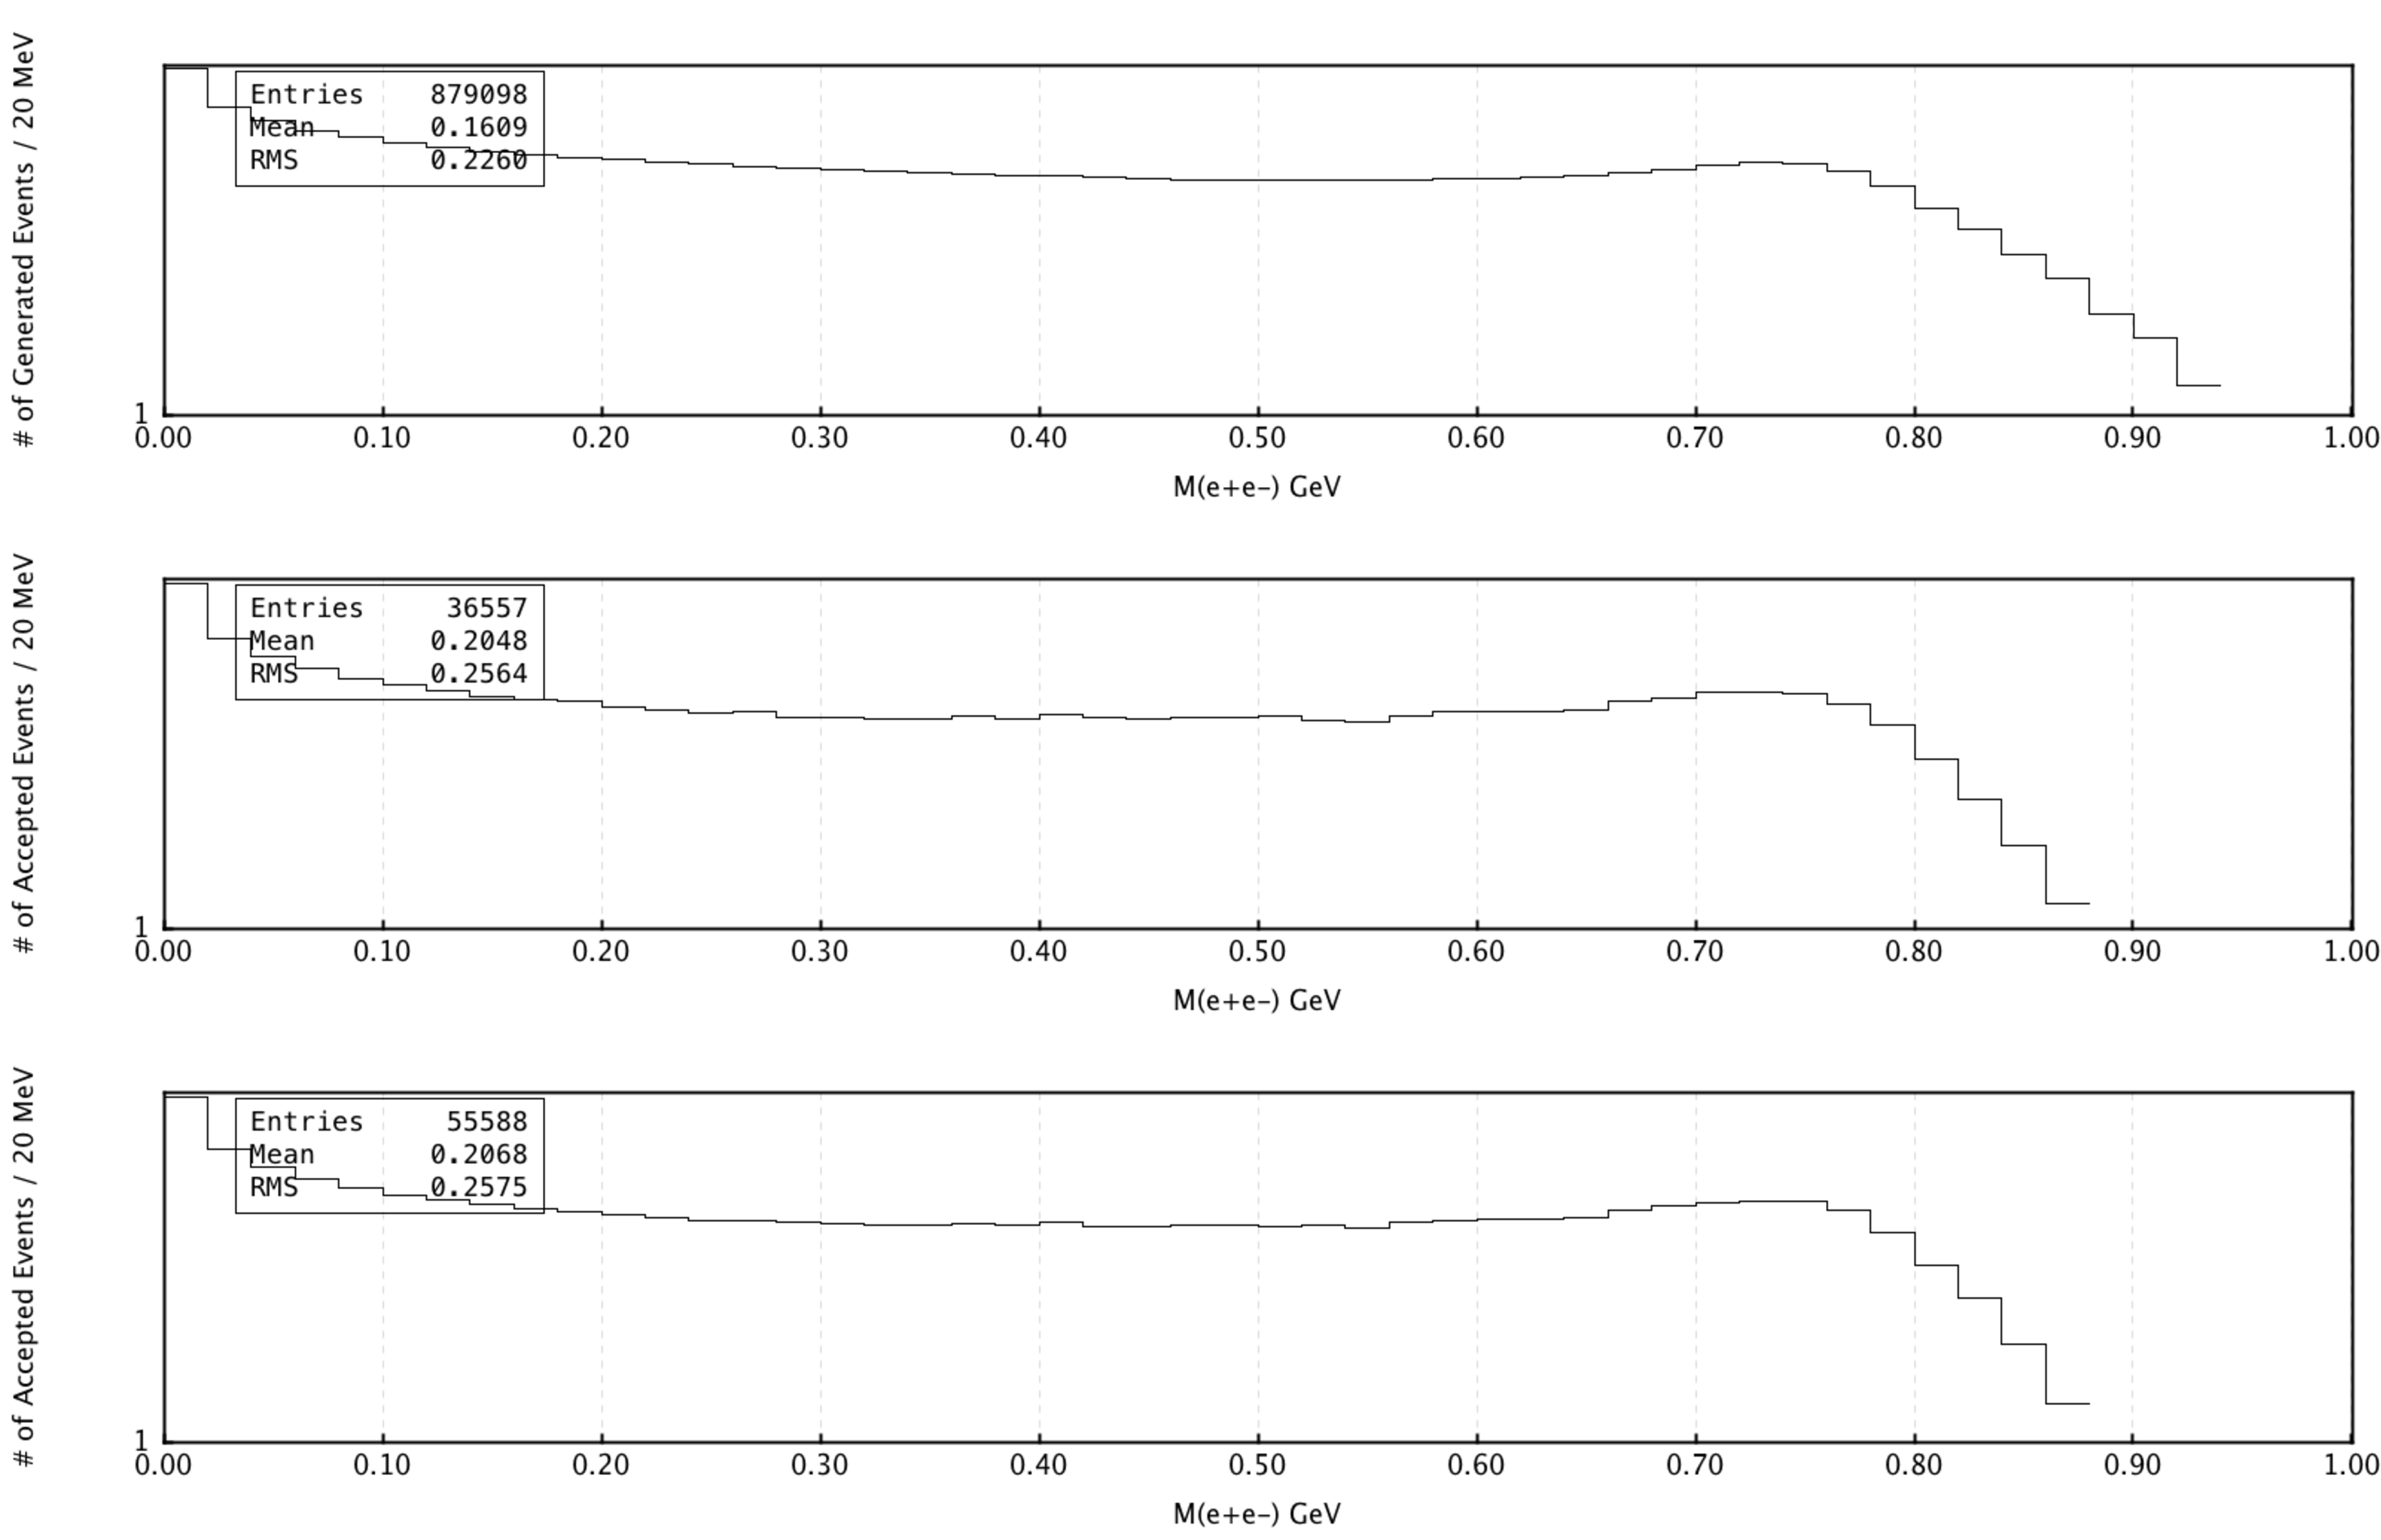
\includegraphics[width=\figwidth,height=2.6\qfigheight]{\grpath/counts/VMD/VMD_Generated_Accepted.pdf}
		\caption[Probability of pair production, $\gamma \to$\epemT, as a function of $M(\epem)$]{\label{fig:VMD}{Probability of pair production in 1~mm of  $\ell H_2$ for $\etaP \to \gamma \gamma $ and $\phi \to \gamma \eta$  vs. $M(\epem)$}}
\end{center}\end{figure}


\begin{figure}[h!]\begin{center}
		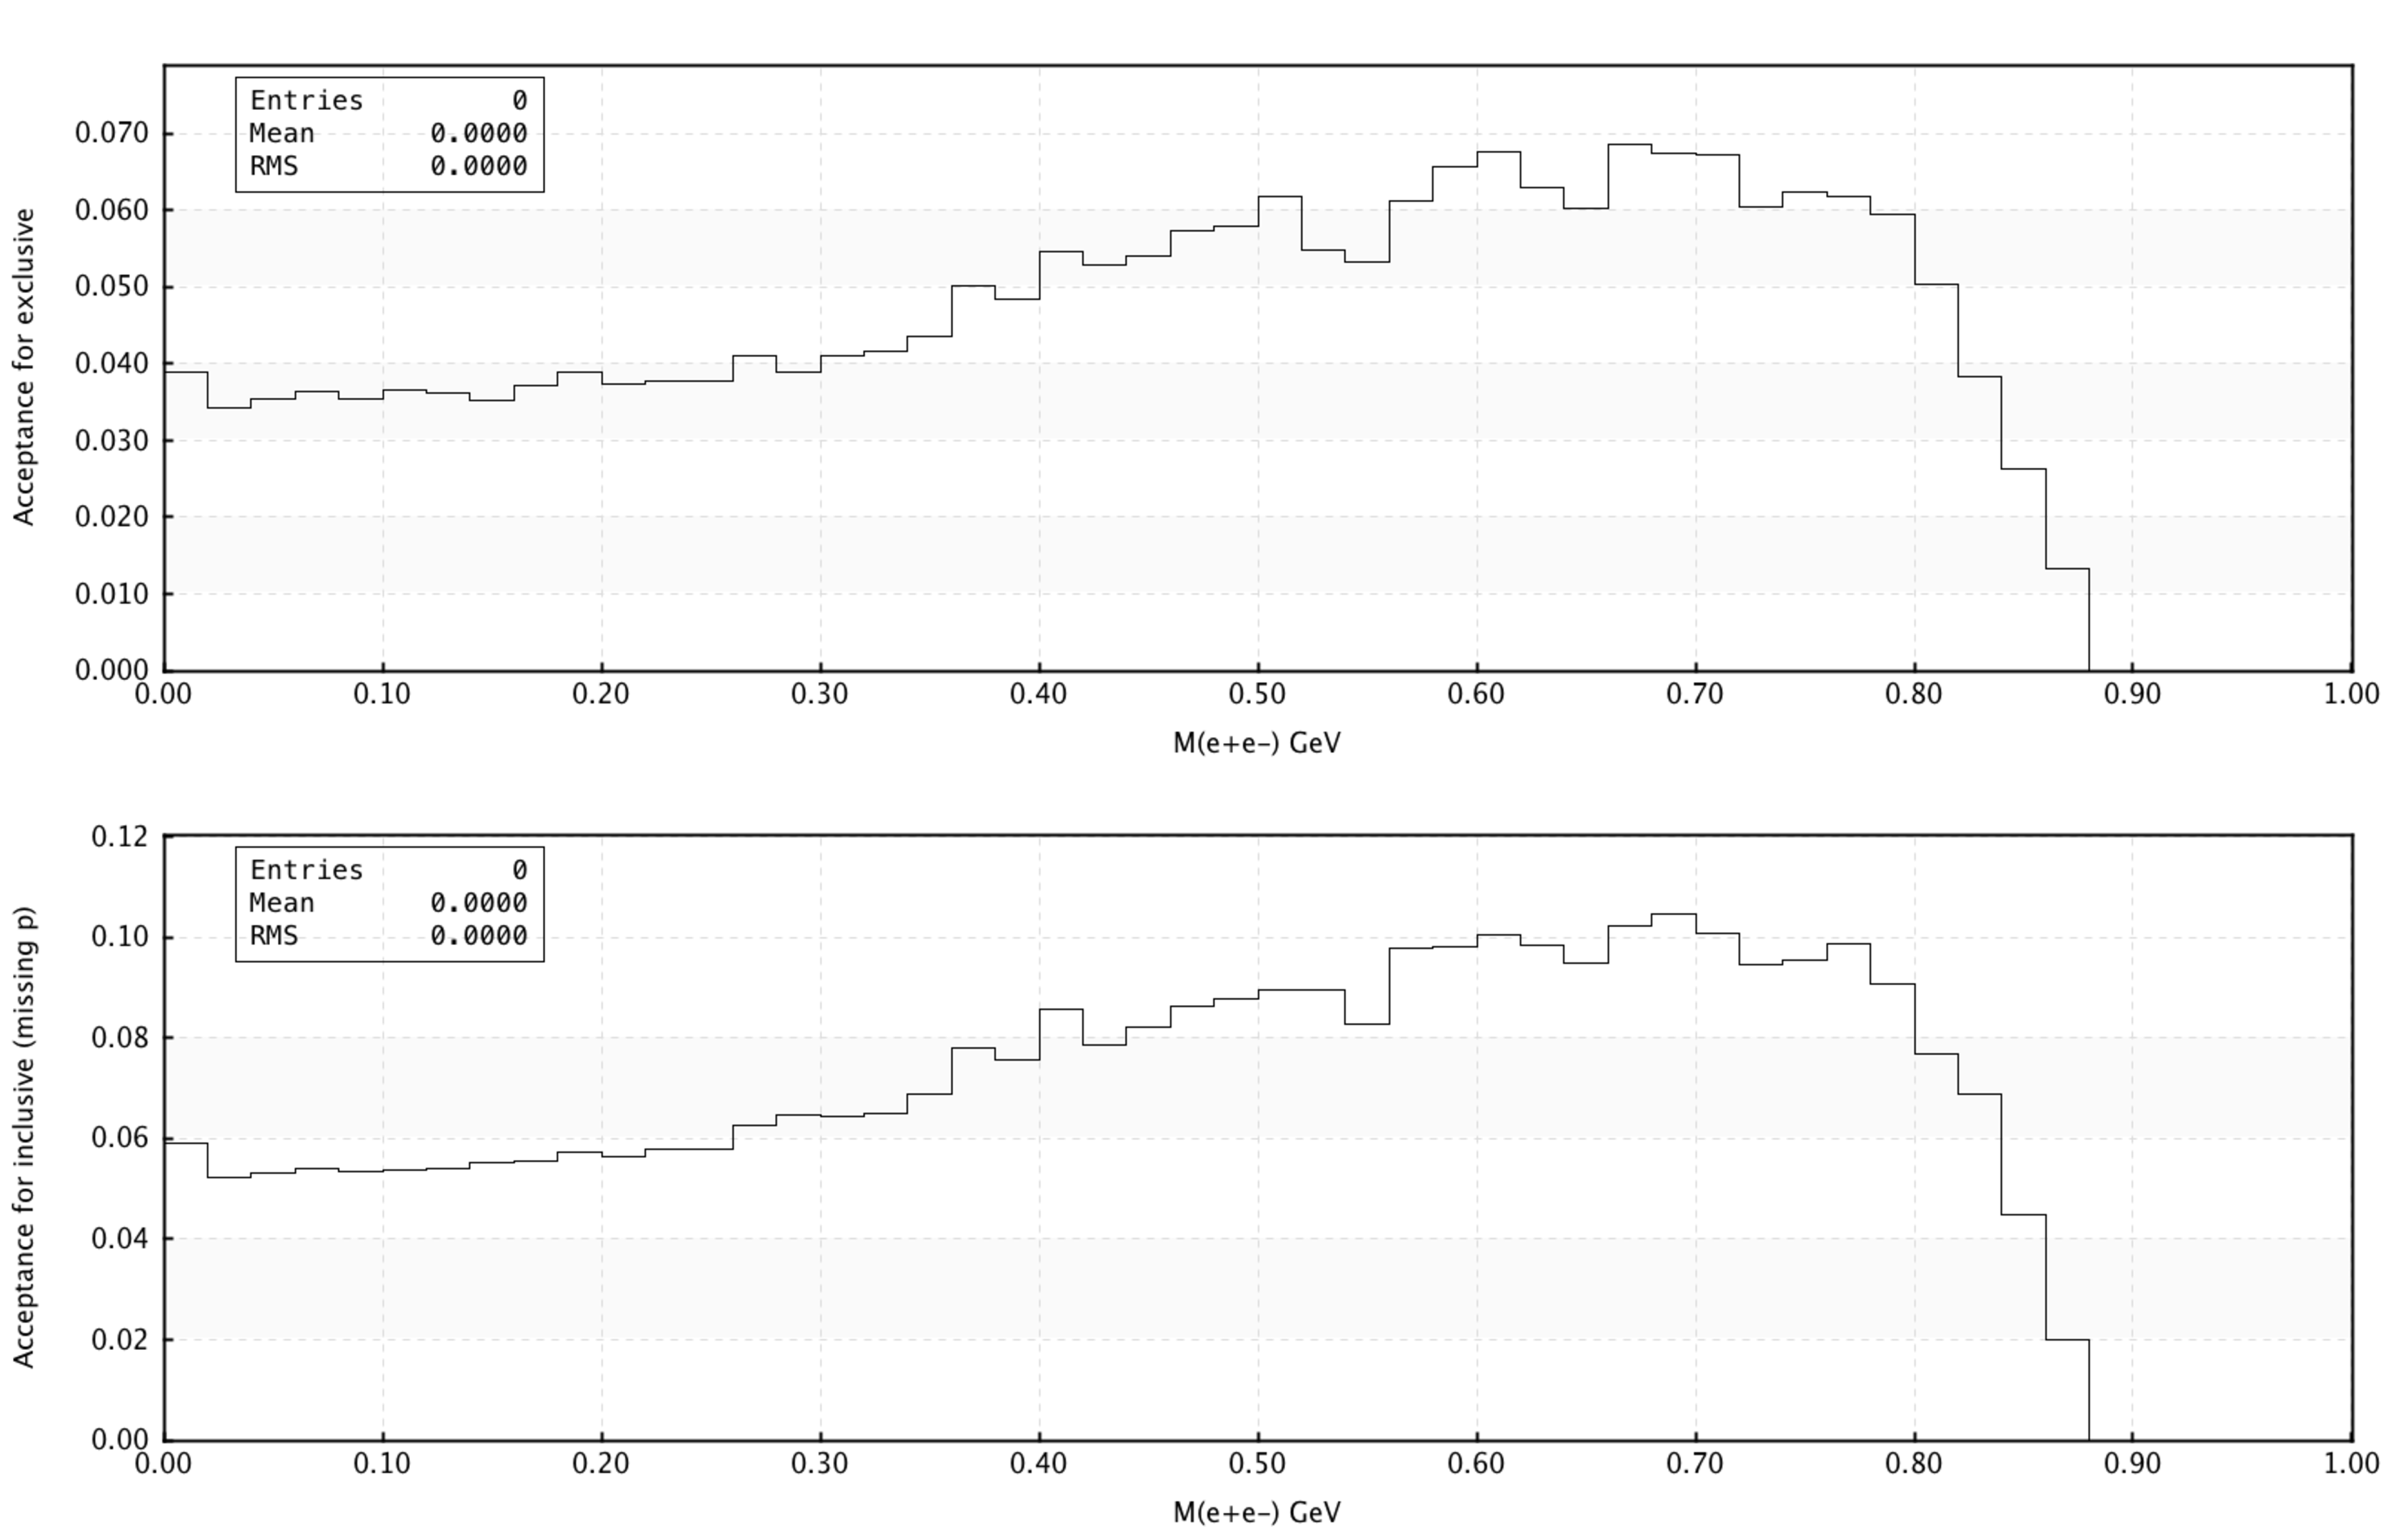
\includegraphics[width=\figwidth,height=1.2\qfigheight]{\grpath/counts/VMD/VMD_Acceptance.pdf}
		\caption[Probability of pair production, $\gamma \to$\epemT, as a function of $M(\epem)$]{\label{fig:conversion_inM}{Probability of pair production in 1~mm of  $\ell H_2$ for $\etaP \to \gamma \gamma $ and $\phi \to \gamma \eta$  vs. $M(\epem)$}}
\end{center}\end{figure}


Checking acceptance by generating a flat $M(\epem)$ mass distribution
 \begin{figure}[h!]\begin{center}
 		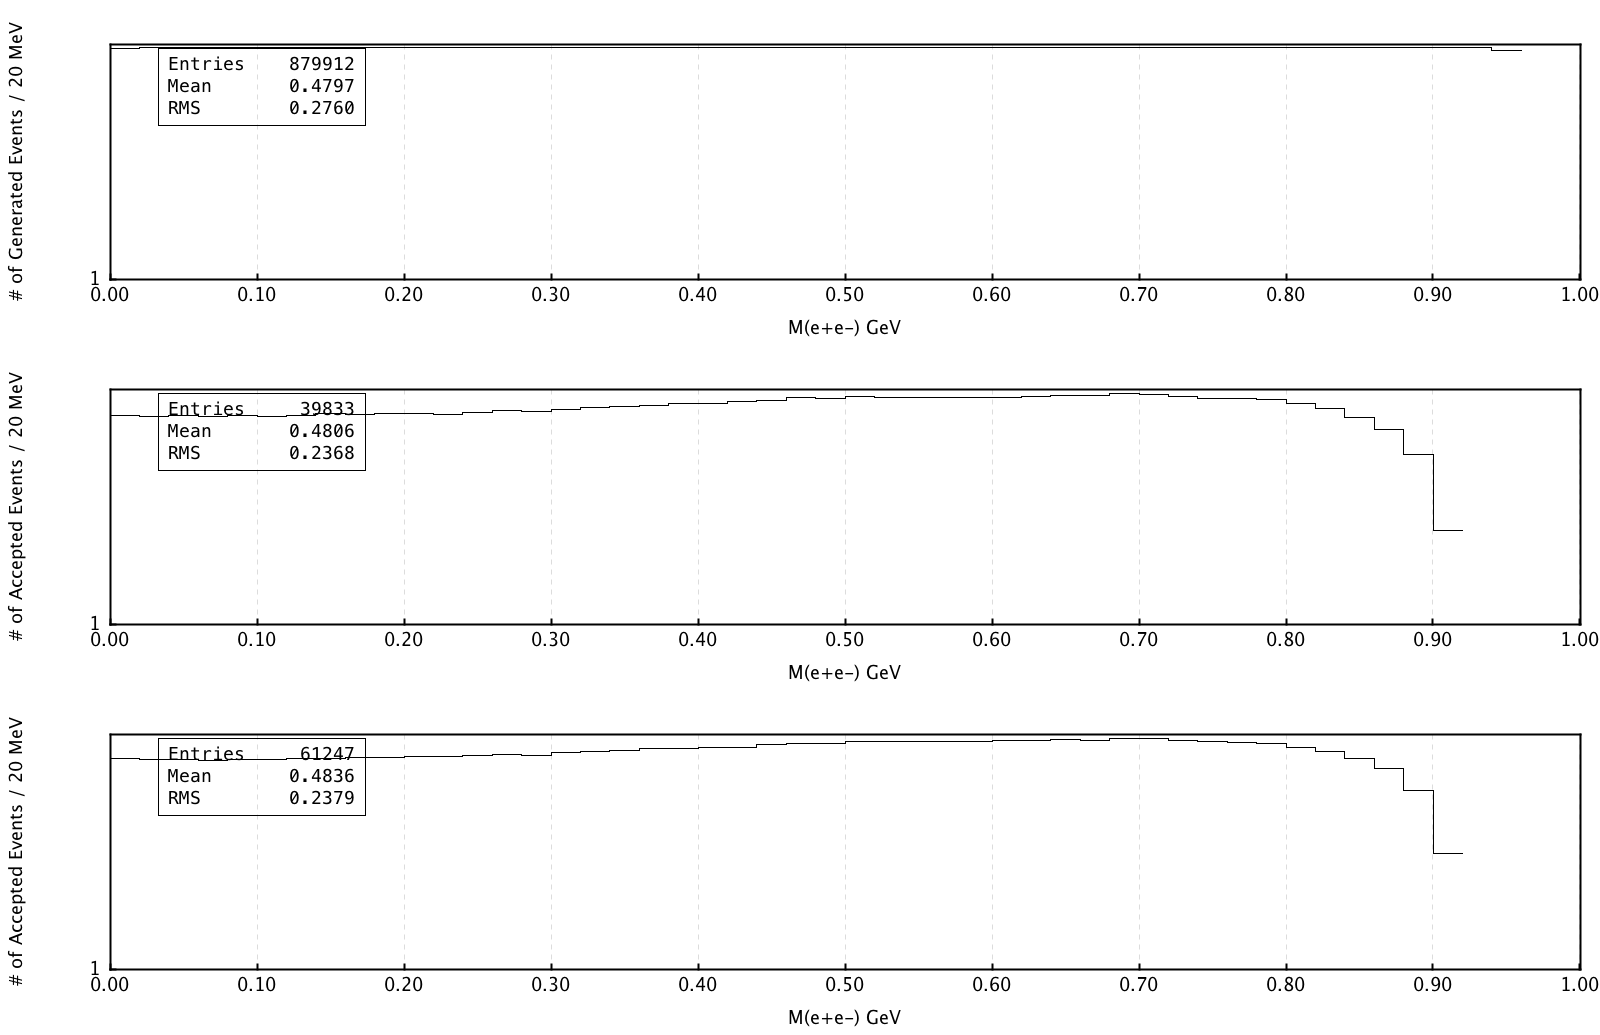
\includegraphics[width=\figwidth,height=2.6\qfigheight]{\grpath/counts/FLAT/FLAT_Generated_Accepted.png}
 		\caption[Probability of pair production, $\gamma \to$\epemT, as a function of $M(\epem)$]{\label{fig:conversion_inM}{Probability of pair production in 1~mm of  $\ell H_2$ for $\etaP \to \gamma \gamma $ and $\phi \to \gamma \eta$  vs. $M(\epem)$}}
 \end{center}\end{figure}
 
 
 \begin{figure}[h!]\begin{center}
 		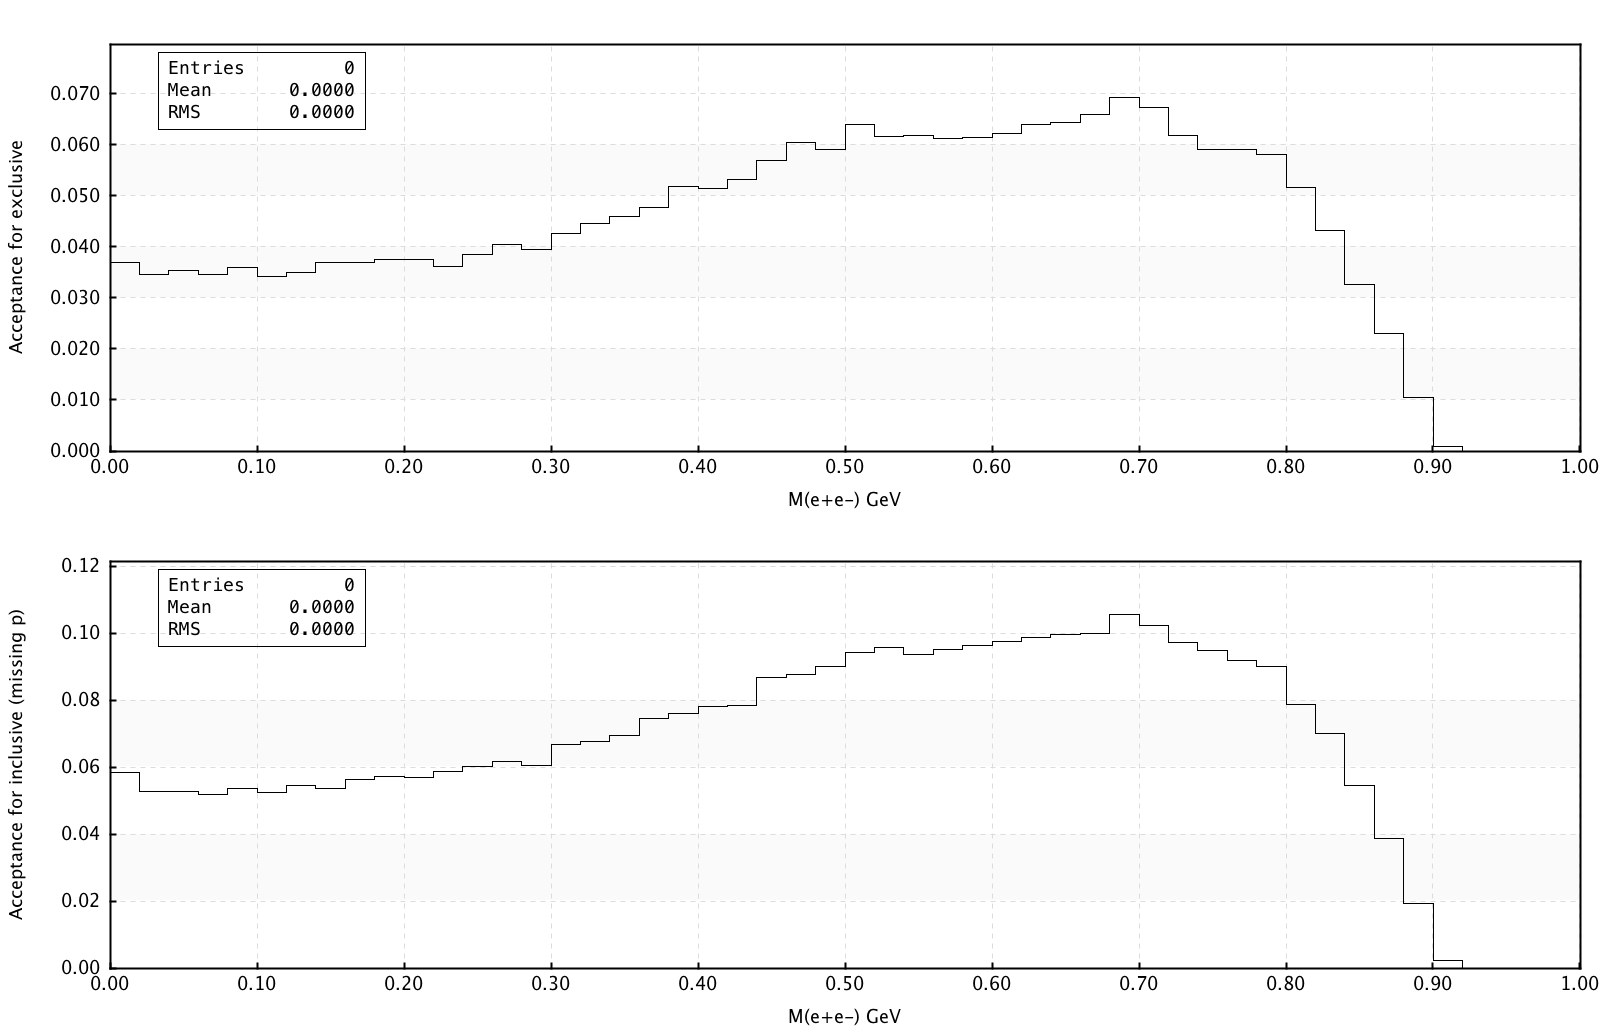
\includegraphics[width=\figwidth,height=1.2\qfigheight]{\grpath/counts/FLAT/FLAT_Acceptance.png}
 		\caption[Probability of pair production, $\gamma \to$\epemT, as a function of $M(\epem)$]{\label{fig:conversion_inM}{Probability of pair production in 1~mm of  $\ell H_2$ for $\etaP \to \gamma \gamma $ and $\phi \to \gamma \eta$  vs. $M(\epem)$}}
 \end{center}\end{figure} 

\subsection{Calculating Expected Yield}
\subsubsection{Calculating Photon Flux}\label{sec:calflux}
A simple method for calculating the photon flux in CLAS12 is as follows; Using the fact that g12 had a photon flux of $7\cdot 10^7 \mathrm{\gamma/s}$ on a Au radiator of $10^{-4} \chi_0$ an expected $\sim 4\cdot 10^9  \mathrm{\gamma/s}$ will be seen in CLAS12 at ${\cal L} = 10^{35}\mathrm{cm^{-2}s^{-1}}$ on a 5~cm $\ell H_2$ target which is $\sim 5.7\cdot 10^{-3} \chi_0$. This number has been independently confirmed in a previous CLAS proposal~\cite{clas.proposal.meson}.
\subsubsection{Calculating Yield}
The average number of \etaDal \ expected in CLAS12 can be calculated as:
Table~\ref{tab:counts} in App.~\ref{sec:app.rates} depicts the upper and lower amount of \epemT expected from 80 days of beam time.




\begin{align}
\bar{N}(\epem)_{\etaP \to \epem \gamma} = \Phi \epsilon(\epem)\bar{\sigma} \rho_{\ell_{H_2}}\ell_{target}N_A \frac{\Gamma_{\mathrm{tot} \etaP}}{\Gamma_{\etaP \to \epem \gamma}}\ ,
\end{align}
where $\Phi$ is the photon flux estimated in Sec.~\ref{sec:calflux}, $\epsilon$ is the acceptance, $\bar{\sigma}$ is the average cross-section, $\rho_{\ell_{H_2}}$ is the atomic density of $\ell_{H_2}$, $\ell_{target}$ is the target length, $N_A$ is Avogadro's constant, and $\frac{\Gamma_{\mathrm{tot} \etaP}}{\Gamma_{\etaP \to \epem \gamma}}$ is the total branching fraction of \etaTP \  decaying into $\epem \gamma$.
Using the lepton acceptance shown is Sec.~\ref{sec.acceptance} the average number of \etaTP \  per $M(\epem)$ can be seen in Fig.~\ref{fig:etayield}.
 \begin{figure}[h!]\begin{center}
 \subfloat[$\etaP$ Dalitz and conversion spectra][]{ %Feynman diagram of $\etaP$ two photon decay
	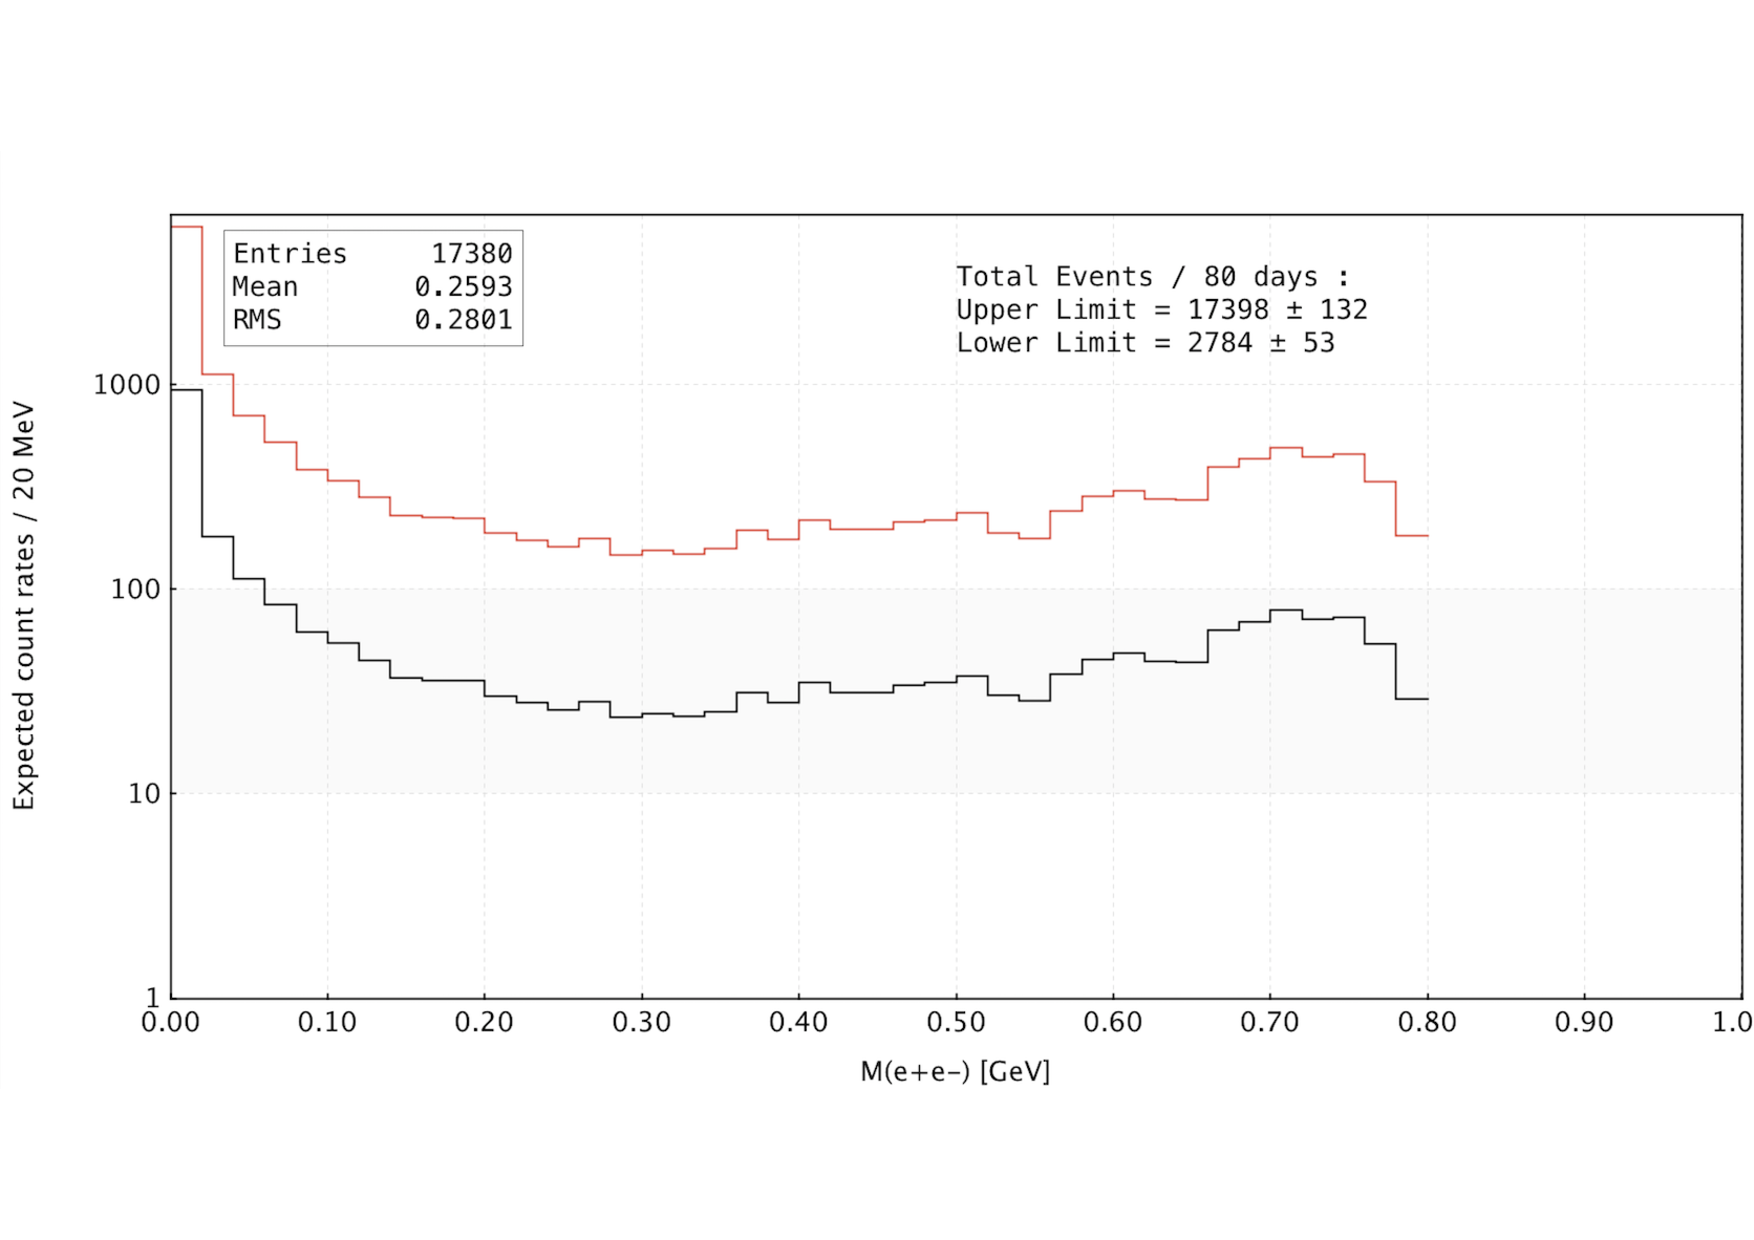
\includegraphics[width=0.8\columnwidth,height=1.0\qfigheight]{\grpath/counts/VMD/VMD_Excluvise_count_rate.pdf}\label{fig:etap_count_exclu}
	}
\\
\subfloat[$\phi$ Dalitz and conversion spectra][]{ %Feynman diagram of $\etaP$ Dalitz decay
	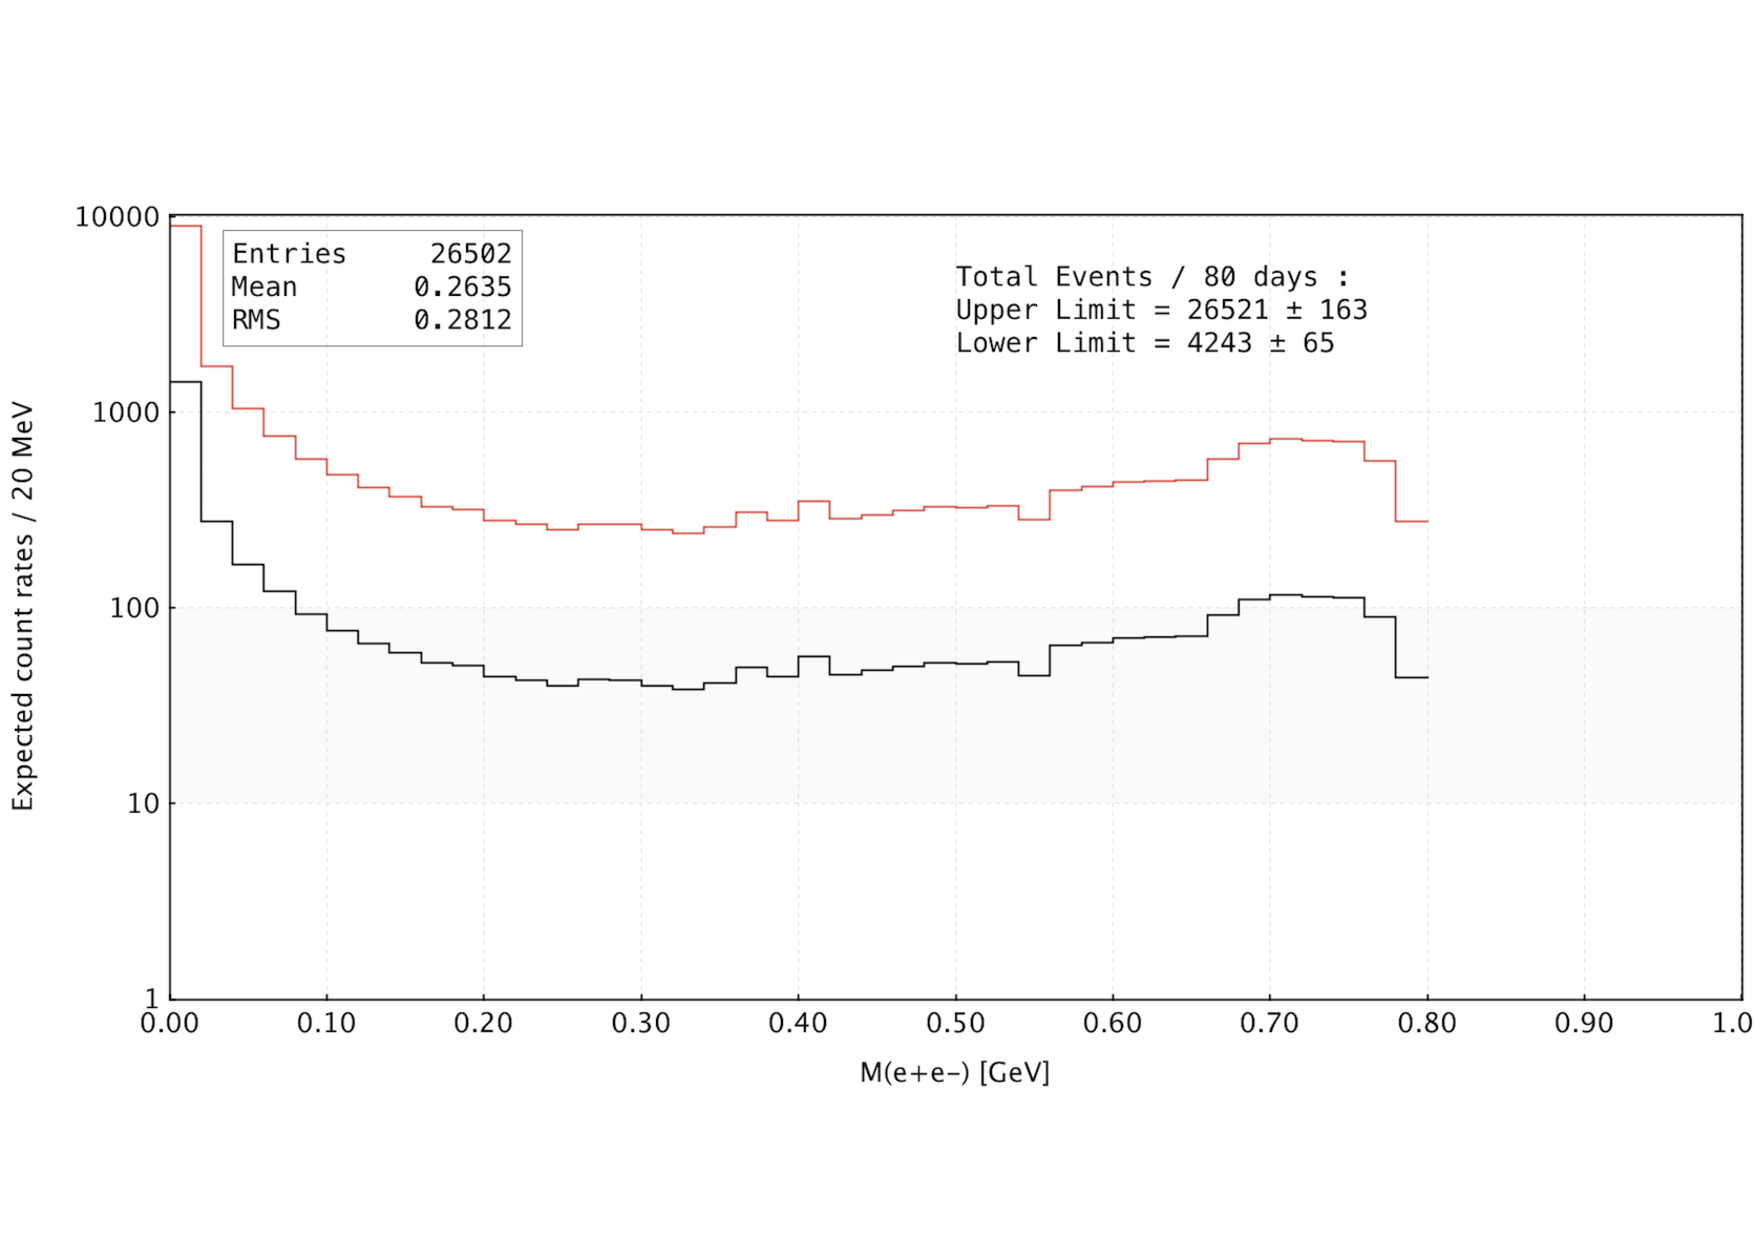
\includegraphics[width=0.8\columnwidth,height=1.0\qfigheight]{\grpath/counts/VMD/VMD_Incluvise_count_rate.pdf}\label{fig:etap_count_exclu}
	}
\caption[Dalitz and conversion spectra for \etaTP \ and $\phi$]{\label{fig:etayield}Example of Dalitz and conversion spectra for \etaTP \ with 500K Dalitz events generated and $\sim 2.35 \cdot 10^7$ $\etaP \to \gamma \gamma$ generated~\subref{fig:etap_dalitz_w_conversion}.  Example of Dalitz and conversion spectra for $\phi$  with 500K Dalitz events generated and $\sim 5.7 \cdot 10^7$ $\phi \to \eta \gamma$ generated ~\subref{fig:phi_dalitz_w_conversion}. }
\end{center}\end{figure}\\
Integrating the $M(\epem)$ expected yield calculates to be $\sim 30,414$ events for inclusive $ep\to e'\etaP (p) \to e'\epem \gamma(p)$ and $\sim 3,415$ events for exclusive $ep\to e'\etaP p \to e'\epem \gamma p$, and increase of $\sim$35 and $\sim$3.5 respectively to the most statistically reported data sample by BESIII. 

\FloatBarrier
\subsection{Realistic Yield}
As a reality check, lets compute the number of $\etaP \to \epem \gamma$ that g12 would have seen, had the experiment ran for 80 days with the \epemT trigger configuration with a real photon flux as calculated for CLAS12.
The 89 $\etaP \to \epem \gamma$ events produced in g12 were recorded when the \epemT trigger was established. This time was 66\% of the total 44 days, which is $\sim29$ days. The total integrated flux measured during this time was $\sim 8.8\cdot 10^{13} \gamma \mathrm{'s}$, therefore in 80 days the total integrated flux would have been $\sim 2.4\cdot 10^{14}$ and the total number of \etaPDal \ events recorded would have been 242. The ratio of g12 total flux at 80 days per CLAS12 real photon flux is $2.73\cdot 10^{16} / 2.4\cdot 10^{14} \sim 114 $. Therefore g12 would have recorded $114\cdot 242 = 27590$ \etaPDal events, which is consistent with what is proposed to be measured in the inclusive measurement of the analysis.